\documentclass[11pt,letter]{ivoa}
\input tthdefs

\usepackage{listings}
\lstloadlanguages{XML}
\lstset{flexiblecolumns=true,basicstyle=\footnotesize,tagstyle=\ttfamily,showspaces=false}

\title{IVOA Support Interfaces}

\ivoagroup{Grid and Web Services Working Group}

\author{Grid and Web Services Working Group}

\editor{Matthew Graham}
\editor{Guy Rixon}
\editor{Patrick Dowler}
\editor{Brian Major}

\previousversion[http://www.ivoa.net/documents/VOSI/20110531/REC-VOSI-1.0-20110531.html]{VOSI-1.0}

\begin{document}
\begin{abstract}
This document describes the minimum interface that a web service requires to participate in the IVOA. Note that this is not required of standard VO services developed prior to this specification, although uptake is strongly encouraged on any subsequent revision. All new standard VO services, however, must feature a VOSI-compliant interface. 
\end{abstract}


\section*{Acknowledgments}

This document has been developed with support from the National Science Foundation's Information Technology Research Program under Cooperative Agreement AST0122449 with The Johns Hopkins University, from the UK Particle Physics and Astronomy Research Council (PPARC), from the European Commission's (EC) Sixth Framework Programme via the Optical Infrared Coordination Network (OPTICON), and from EC's Seventh Framework Programme via its eInfrastructure Science Repositories initiative.

This work is based on discussions and actions from the 2003 IVOA meeting in Strasbourg and further discussions on registry functionality at JHU late in 2003. Later inputs came from a local meeting at JHU in Sept. 2004. William O'Mullane and Ani Thakar were the editors and primary authors for these early versions.

The decision to split the interfaces into a mandatory set and optional logging interfaces was taken by GWS-WG at the IVOA meeting of May 2006. 

\section*{Conformance-related definitions}

The words ``MUST'', ``SHALL'', ``SHOULD'', ``MAY'', ``RECOMMENDED'', and
``OPTIONAL'' (in upper or lower case) used in this document are to be
interpreted as described in IETF standard RFC2119 \citep{std:RFC2119}.

The \emph{Virtual Observatory (VO)} is a
general term for a collection of federated resources that can be used
to conduct astronomical research, education, and outreach.
The \href{http://www.ivoa.net}{International
Virtual Observatory Alliance (IVOA)} is a global
collaboration of separately funded projects to develop standards and
infrastructure that enable VO applications.


\section{Introduction}
\label{sec:introduction}

This document describes a set of common basic functions that VO web services provide in the form of a standard support interface in order to allow for the effective management of the VO.  There are three basic support functions that this document describes:  The reporting of capability metadata, the reporting of service availability metadata, and the reporting of table metadata (if applicable).

VO service standards previous to VOSI may not be forced to retrospectively implement VOSI (although that should be encouraged). Nonetheless, all new VO service standards (or updated existing ones) must enforce the VOSI implementation.


\subsection{Role within the VO Architecture}

The IVOA Architecture \citep{note:VOARCH} provides a high-level view of how IVOA standards work together to connect users and applications with providers of data and services, as depicted in the diagram in Figure ~\ref{fig:archdiag}. 

\begin{figure}
\centering


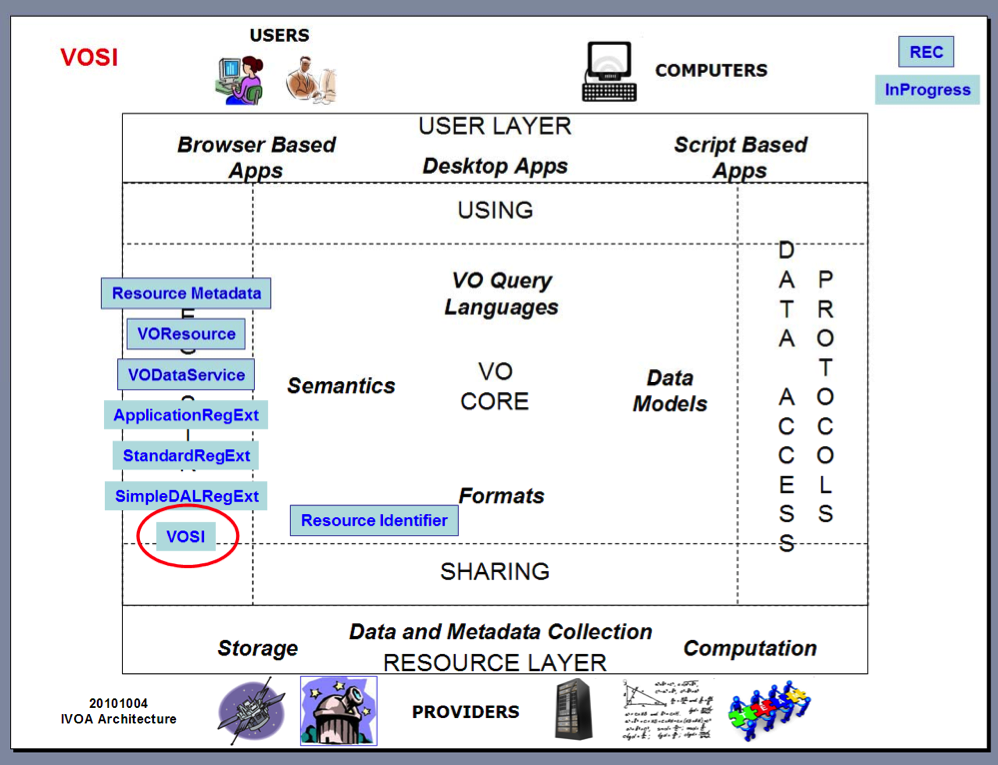
\includegraphics[width=0.9\textwidth]{archdiag.png}
\caption{VOSI in the IVOA Architecture. VOSI is the standard that defines the basic functions that all VO services should provide in order to support management of the VO.}
\label{fig:archdiag}
\end{figure}

In this architecture, users employ a variety of tools (from the User
Layer) to discover and access archives and services -- that is,
resources -- of interest (represented in the Resource Layer). A registry
plays a role in discovery by harvesting metadata that describe archives
and services and making them searchable from a central service. The VOSI
interface provides a means for a service to provide some of this
metadata itself; this allows a registry to pull the metadata from the
service rather than relying on a human to provide it (e.g. by typing the
data into a registration form manually). This mechanism can make it
easier to collect highly detailed metadata (e.g. descriptions of columns
in a catalog) that might not be practically provided otherwise. As some
of this metadata describes the service interface and how it behaves,
other applications can use this information for controlling how they use
the service. Even when the service is ``discovered'' through some means other than a registry, an application can still understand how to use the service by querying for this information directly. (See Appendix \ref{appendix:harvesting} for a more detailed description of this use case.)

Once a user discovers data and services of interest, she will want to engage them in an analysis process. Success requires that the selected services are actually up and running properly as a down service can cause automated processing to fail completely. Registry and workflow services can assist with this by tracking the availability of services and alerting users about downtime. We envision that VOSI will allow VO projects to better track the overall health of the VO ecosystem. 

\section{Interface bindings}
\label{sec:bindings}

The standard interface returns metadata without changing the state of the service with which it is associated. This standard requires a REST binding of VOSI even when applied to services that do not have a RESTful interface.

In the REST binding, the support interfaces shall have distinct URLs in the HTTP scheme and shall be accessible by the GET operation in the HTTP protocol. The response to an HTTP POST, PUT or DELETE to these resources is not defined by this specification. However, if an implementation has no special action to perform for these requests, the normal response would be a HTTP 405 "Method not allowed" status code.

The endpoints and interface types for the support interface shall be defined in the service's registration using one \xmlel{capability} element for each interface. The values of the \xmlel{standardID} attribute for these Capabilities are given in section~\ref{sec:endpoints}.

When using the REST binding, any HTTP URLs may be used. The client must find the appropriate URLs from the service's entry in the VO registry and, in general, should not try and infer the URLs from any other URLs for that service. However, standards for specific services may put extra constraints on the form of the URLs.

\section{Metadata specification}
\label{sec:metadata}

 There are various classes of metadata that might be returned by a service through its standard interface:

\begin{itemize}
\item those describing its functional capabilities
\item those describing its operational behaviour - availability, reliability, etc.
\item those describing tabular data handled by the service
\item those describing other aspects of the service 
\end{itemize}

This section defines how each of these classes is represented. The following typographic convention is used to represent a XML element defined within a particular namespace:

$$\hbox{\xmlel{http://some.name.space\#elementName}}$$

For example, \xmlel{http://www.ivoa.net/xml/VOResource/v1.0\#resource} indicates a XML element named \xmlel{resource} that is described in the XML schema associated with the 'http://www.ivoa.net/xml/VOResource/v1.0' namespace -- in this case, this would be VOResource.xsd \citep{std:VOR}. 

\subsection{Capability metadata}

Note:
    'Capability' is unfortunately an overloaded term in the VO referring to both a functional aspect of a service and also particular pieces of metadata defined by various XML schema. When referring to an XML element called \xmlel{capability}, it shall be typeset in italic typewriter. Its parent namespace may also be included (using the syntax described above) if it is ambiguous which XML schema is being referred to. 
    
This interface provides the service metadata in the form of a list of Capability descriptions. Each of these descriptions is an XML element that:

\begin{itemize}
\item states that the service provides a particular, IVOA-standard function;
\item lists the interfaces for invoking that function;
\item records any details of the implementation of the function that are not defined as default or constant in the standard for that function. 
\end{itemize}

For example, one Capability might describe a cone search function and another the TAP implementation but these two might well apply to the same service.

An entry for a service in the resource registry - i.e., its VOResource - contains the Dublin Core resource metadata (identifier, curation information, content description, etc.) followed by the service's capability descriptions (expressed as a series of \xmlel{http://www.ivoa.net/xml/VOResource/v1.0\#Ca\-pa\-bi\-lity} elements). Effectively, the resource metadata describes the service to human users and the capability list describes it to software. Therefore, the latter list has two uses:

\begin{itemize}
\item it may be read by a client application to find out how to invoke the service. This presumes that the service has been already been selected and the VOSI endpoint located.
\item it may be read by the registry itself to compile the registry entry for the service. In this case, the resource metadata are entered into the registry directly and the service metadata are then read from the service. Since the service implementation usually knows its capabilities, this removes the need for a human to type them into the registry. 
\end{itemize}

The service metadata shall be represented as an XML document with the root element \xmlel{http://www.ivoa.net/xml/VOSICapabilities/v1.0\#capabilities}. (See Appendix \ref{appendix:capabilities} for the definition of the VOSICapabilities XML schema.) This element must contain one or more child capability elements that describe the capabilities of the service. Given that the capability element is defined to be of type \xmlel{http://www.ivoa.net/xml/VOResource/v1.0\#Capability}, a capability element may be represented by a legal sub-type of 
\xmlel{http://www.ivoa.net/xml/VOResource/v1.0\#Capability}, in which case, the capability element must use an \xmlel{xsi:type} attribute to identify the sub-type (see section 2.2.1 of VOResource \citep{std:VOR}). 


\begin{admonition}{Note}
The value of the capability element's \xmlel{standardID} attribute is used to indicate the service's support for particular standard protocols (such as Simple Image Access, Simple Cone Search, etc.). In the case of some protocols, the support for the standard is further characterized by additional metadata provided by a standard XML schema extension of \xmlel{Capability} for that protocol. The extension metadata is enabled by adding a \xmlel{xsi:type} attribute to the capability element set to the Capability sub-type value defined in the extension schema for that protocol (see example below). 
    
The VOResource list of capabilities should include capabilities describing VOSI endpoints as specified in section \ref{sec:endpoints}.
\end{admonition}

In the REST binding, the service metadata shall be a single web resource with a registered URL. The date and time at which the metadata last changed shall be obtained from the Last-Modified HTTP Header keyword sent in the response to a GET or HEAD request to the registered URI.

All VO services should provide this interface. 

\subsection{Non-service metadata (non-normative)}

There may be other metadata associated with a service than the capability metadata described above.

\begin{itemize}
\item Every service has the Dublin Core resource metadata \citep{std:DUBLINCORE}.
\item Some services are associated with registered applications.
\item Some services are associated with registered data collections. 
\end{itemize}

None of these are explicitly provided for in this version of VOSI. Some might be covered in later versions of VOSI. 

\subsection{Availability metadata}

This interface indicates whether the service is operable and the reliability of the service for extended and scheduled requests. The availability shall be represented as an XML document in which the root element is \xmlel{http://www.ivoa.net/xml/Availability/v1.0\#availability}. This element shall contain child elements providing the following information:

\begin{itemize}
\item \xmlel{available} -- whether the service is currently accepting requests
\item \xmlel{upSince} -- duration for which the service has been continuously available
\item \xmlel{downAt} -- the instant at which the service is next scheduled to be unavailable
\item \xmlel{backAt} -- the instant at which the service is scheduled to become available again after down time;
\item \xmlel{note} -- textual note, e.g. explaining the reason for unavailability. 
\end{itemize}

The elements \xmlel{upSince}, \xmlel{downAt}, \xmlel{backAt} and \xmlel{note} are optional. The \xmlel{available} element is mandatory. There may be more than one \xmlel{note} element.

The XML document shall conform to the schema given in appendix \ref{appendix:availability} of this specification.

When reporting availability, the service should do a good check on its underlying parts to see if it is still operational and not just make a simple return from a web server, e.g., if it relies on a database it should check that the database is still up. If any of these checks fail, the service should set available to false in the availability output.

If a service is to be online but unavailable for work (e.g., when a service with a work queue intends to shut down after draining the queue) then the service should set available to false.

There are no special elements in the availability document for the contact details of the service operator. These details may be given as a note element if they are known to the service.

In the REST binding, the availability shall be a single web resource with a registered URL

All VO services shall provide this interface. 

\subsection{Table metadata}

 Some services deal with tabular data. These data may be the target of ADQL queries, as in TAP \citep{std:TAP}, or they may be the output of other operations, as in SIAP queries. In each case, it is useful if the service describes the details of the tables concerned. It is more useful if this description can be captured in the resource registry.

The VODataService standard \citep{std:VODS11} defines XML elements for describing a set of tables. These elements can be included in a resource document for a service.

A service which uses tables in its interface should define a VOSI endpoint from which table metadata can be read. The table metadata for all content of a service shall be represented as an XML document of which the root element is of type 
\xmlel{http://www.ivoa.net/xml/VODataService/v1.1\#TableSet}. The table metadata for a single table (see below) shall be represented as an
XML document of which the root element is of type \xmlel{http://www.ivoa.net/xml/VODataService/v1.1\#Table}. This element may contain any mix of elements allowed by the VODataService XML schema.

In the REST binding, the TableSet metadata shall be a hierarchical web resource with a registered URL.  There are two levels of TableSet metadata detail that may be returned from the base \textit{tables} endpoint.  Maximum detail (max) is the complete metadata including all details of the Table elements.  Minimum detail (min) includes the full set of Table elements with names and optional descriptions, but does not include Table elements of type Column or ForeignKey.

If the parameter \textit{detail} accompanies the request with values of either \textit{max} or \textit{min}, the service should take this as a suggestion as to what level of detail to return, but may return either level.  If the parameter \textit{detail} is not present, the service may choose the level of metadata detail to return.

For example, the request:

\begin{verbatim}
GET http://example.net/srv/tables?detail=min
\end{verbatim}

should be taken as a suggestion to return the minimum level of TableSet metadata detail.

Services with a large number of tables and/or columns cannot normally respond with a usable TableSet document that has the maximum level of detail so may wish to always respond with the minimum level of detail.

The REST endpoint must also support a child resource for each table described in the TableSet document.  The child resource must be named as it appears in the name of the corresponding child Table element.  For example:

\begin{verbatim}
GET http://example.net/srv/tables/ivoa.ObsCore
\end{verbatim}

would return a Table document describing the ivoa.ObsCore table in full detail, starting:

\begin{verbatim}
<vosi:table xmlns:vosi="http://www.ivoa.net/xml/VOSITables/v1.0">
    <name>ivoa.ObsCore</name>
    <column>
    ...
\end{verbatim} 

\section{Registration of VOSI endpoints}
\label{sec:endpoints}

The endpoints for the service and availability metadata shall be included in the registration of each service that provides them.

\begin{tabular}{l l l l l}
\label{tab:registration}
Endpoint type & standardID value \\
availability & \nolinkurl{ivo://ivoa.net/std/VOSI#availability} \\
capabilities & \nolinkurl{ivo://ivoa.net/std/VOSI#capabilities} \\
tables (1.0) & \nolinkurl{ivo://ivoa.net/std/VOSI#tables} \\
tables (1.1) & \nolinkurl{ivo://ivoa.net/std/VOSI#tables-1.1} \\
\end{tabular}

An availability endpoint shall be represented by an element named \xmlel{capability}, of type \xmlel{http://www.ivoa.net/xml/VOResource/v1.0\#Capability} (defined by the standard VOResource XML schema \citet{std:VOR}). The value of the \xmlel{standardID} attribute of the capability shall be \nolinkurl{ivo://ivoa.net/std/VOSI#availability}.

A capabilities endpoint should be represented by an element named \xmlel{capability}, of type \xmlel{http://www.ivoa.net/xml/VOResource/v1.0\#Capability}. If such a capability is provided then the value of the \xmlel{standardID} attribute must be \nolinkurl{ivo://ivoa.net/std/VOSI#capabilities}.

A tables endpoint should be represented by an element named \xmlel{capability}, of type \xmlel{http://www.ivoa.net/xml/VOResource/v1.0\#Capability}. If such a capability is provided then the value of the \xmlel{standardID} attribute must be \nolinkurl{ivo://ivoa.net/std/VOSI\#tables}.

With all three VOSI functions, the \xmlel{capability} element that describes the function must contain an \xmlel{interface} element of a type semantically appropriate for the binding of the function to the service; the \xmlel{accessURL} element within the \xmlel{interface} element indicates the endpoint for the VOSI function. For the REST binding, this \xmlel{accessURL} element must set the \xmlel{use} attribute to \texttt{"full"}. Furthermore, for the REST binding, this document recommends using the \xmlel{http://www.ivoa.net/xml/VODataService/v1.1\#ParamHTTP} interface type to encode VOSI endpoints (see the examples given in section~\ref{sec:examples}). 

The capabilities and availability endpoints must not require any credentials to view.  Thus, the \xmlel{interface} registry entries for capabilities and availability must not contain a securityMethod element.

\section{Example VOSI responses}
\label{sec:examples}

\subsection{Example 1: SIA 1.0 capabilities}

A sample response from a capabilities resource describing an SIA service. 

\begin{lstlisting}[language=XML,basicstyle=\footnotesize]
<?xml version="1.0" encoding="UTF-8"?>
<vosi:capabilities xmlns:vosi="http://www.ivoa.net/xml/VOSICapabilities/v1.0"
    xmlns:vr="http://www.ivoa.net/xml/VOResource/v1.0"
    xmlns:vs="http://www.ivoa.net/xml/VODataService/v1.0"
    xmlns:sia="http://www.ivoa.net/xml/SIA/v1.0"
    xmlns:xsi="http://www.w3.org/2001/XMLSchema-instance"
    xsi:schemaLocation="http://www.ivoa.net/xml/VOSI/v1.0 
        http://www.ivoa.net/xml/VOSI/v1.0
      http://www.ivoa.net/xml/VOResource/v1.0 
        http://www.ivoa.net/xml/VOResource/v1.0
      http://www.ivoa.net/xml/VODataService/v1.0 
        http://www.ivoa.net/xml/VODataService/v1.0
      http://www.ivoa.net/xml/SIA/v1.0 
        http://www.ivoa.net/xml/SIA/v1.0">

  <!-- a generic capability (for custom, non-standard interfaces) -->
  <capability>
    <interface xsi:type="vr:WebBrowser">
      <accessURL use="full"> http://adil.ncsa.uiuc.edu/siaform.html 
      </accessURL>
    </interface>
  </capability>
  
  <!-- the SIA capability -->
 
  <capability xsi:type="sia:SimpleImageAccess" 
      standardID="ivo://ivoa.net/std/SIA">
    <interface xsi:type="vs:ParamHTTP" role="std">
      <accessURL> http://adil.ncsa.uiuc.edu/cgi-bin/voimquery?survey=f&amp; 
      </accessURL>
    </interface>

    <imageServiceType>Pointed</imageServiceType>

    <maxQueryRegionSize>

      <long>360.0</long>

      <lat>180.0</lat>

    </maxQueryRegionSize>

    <maxImageExtent>

      <long>360.0</long>

      <lat>180.0</lat>

    </maxImageExtent>

    <maxImageSize>

      <long>5000</long>

      <lat>5000</lat>

    </maxImageSize>

    <maxFileSize>100000000</maxFileSize>

    <maxRecords>5000</maxRecords>

  </capability>

  <!-- the interface that returns this capability -->
  <capability standardID="ivo://ivoa.net/std/VOSI#capabilities">
    <interface xsi:type="vs:ParamHTTP" role="std">
      <accessURL use="full"> 
        http://adil.ncsa.uiuc.edu/cgi-bin/voimquery/capabilities 
      </accessURL>
    </interface>
  </capability>

  <!-- the interface that returns this availability-->
  <capability standardID="ivo://ivoa.net/std/VOSI#availability">
    <interface xsi:type="vs:ParamHTTP" role="std">
      <accessURL use="full"> 
        http://adil.ncsa.uiuc.edu/cgi-bin/voimquery/availability 
      </accessURL>
    </interface>
  </capability>

</vosi:capabilities>
\end{lstlisting}


\subsection{Example 2: TAP tables, maximum detail}

A sample response from a tables resource describing a TAP service in full (maximum) detail.

\begin{lstlisting}[language=XML]
<?xml version="1.0" encoding="UTF-8"?>
<vosi:tableset
  xmlns:vosi="http://www.ivoa.net/xml/VOSITables/v1.0"
  xmlns:xsi="http://www.w3.org/2001/XMLSchema-instance"
  xmlns:vod="http://www.ivoa.net/xml/VODataService/v1.1">

  <schema>
    <name>cfht </name>
    <table type="output">
      <name>cfht.deepU </name>
      <column>
        <name>cfhtlsID </name>
        <dataType xsi:type="vod:TAP" size="30">adql:VARCHAR </dataType>
      </column>
      <column>
        <name>survey </name>
        <dataType xsi:type="vod:TAP" size="6">adql:VARCHAR </dataType>
      </column>
      <column>
        <name>field </name>
        <dataType xsi:type="vod:TAP" size="2">adql:VARCHAR </dataType>
      </column>
      <column>
        <name>pointing </name>
        <dataType xsi:type="vod:TAP" size="6">adql:VARCHAR </dataType>
      </column>
      <column>
        <name>selectionFilter </name>
        <dataType xsi:type="vod:TAP" size="2">adql:VARCHAR </dataType>
      </column>
    </table>

    <table type="output">
      <name>TAP_SCHEMA.keys </name>
      <column>
        <name>key_id </name>
        <description>unique key to join to TAP_SCHEMA.key_columns 
        </description>
        <dataType xsi:type="vod:TAP" size="64">adql:VARCHAR </dataType>
      </column>
      <column>
        <name>from_table </name>
        <description>the table with the foreign key </description>
        <dataType xsi:type="vod:TAP" size="64">adql:VARCHAR </dataType>
      </column>
      <column>
        <name>target_table </name>
        <description>the table with the primary key </description>
        <dataType xsi:type="vod:TAP" size="64">adql:VARCHAR </dataType>
      </column>
    </table>

  </schema>

</vosi:tableset>
\end{lstlisting}

\subsection{Example 3: Tables, minimum detail}

A sample response from a tables resource with no Column or ForeignKey elements.

\begin{lstlisting}[language=XML]
<?xml version="1.0" encoding="UTF-8"?>
<vosi:tableset
  xmlns:vosi="http://www.ivoa.net/xml/VOSITables/v1.0"
  xmlns:xsi="http://www.w3.org/2001/XMLSchema-instance"
  xmlns:vod="http://www.ivoa.net/xml/VODataService/v1.1">

  <schema>
    <name>cfht </name>
    <table type="output">
      <name>cfht.deepU </name>
    </table>
  </schema>
  
  <schema>
    <name>TAP_SCHEMA</schema>
    <table type="output">
      <name>TAP_SCHEMA.tables </name>
    </table>
    <table type="output">
      <name>TAP_SCHEMA.columns </name>
    </table>
    <table type="output">
      <name>TAP_SCHEMA.keys </name>
    </table>
    <table type="output">
      <name>TAP_SCHEMA.key_columns </name>
    </table>
  </schema>

</vosi:tableset>
\end{lstlisting}

\subsection{Example 4: Child table resource}

A sample response from a child table resource (e.g. http://example.net/srv/tables/TAP\_SCHEMA.columns).

\begin{lstlisting}[language=XML]
<?xml version="1.0" encoding="UTF-8"?>
<vosi:table xmlns:vosi="http://www.ivoa.net/xml/VOSITables/v1.0" 
    xmlns:vod="http://www.ivoa.net/xml/VODataService/v1.1" 
    xmlns:xsi="http://www.w3.org/2001/XMLSchema-instance" type="output">
  <name>TAP_SCHEMA.columns</name>
  <column>
    <name>table_name</name>
    <description>the table this column belongs to</description>
    <dataType xsi:type="vod:TAPType" size="64">VARCHAR</dataType>
  </column>
  <column>
    <name>column_name</name>
    <description>the column name</description>
    <dataType xsi:type="vod:TAPType" size="64">VARCHAR</dataType>
  </column>
  <column>
    <name>utype</name>
    <description>lists the utypes of columns in the tableset</description>
    <dataType xsi:type="vod:TAPType" size="512">VARCHAR</dataType>
  </column>
  <column>
    <name>ucd</name>
    <description>lists the UCDs of columns in the tableset</description>
    <dataType xsi:type="vod:TAPType" size="64">VARCHAR</dataType>
  </column>
  <column>
    <name>unit</name>
    <description>lists the unit used for column values in the tableset</description>
    <dataType xsi:type="vod:TAPType" size="64">VARCHAR</dataType>
  </column>
  <column>
    <name>description</name>
    <description>describes the columns in the tableset</description>
    <dataType xsi:type="vod:TAPType" size="512">VARCHAR</dataType>
  </column>
  <column>
    <name>datatype</name>
    <description>lists the ADQL datatype of columns in the tableset</description>
    <dataType xsi:type="vod:TAPType" size="64">VARCHAR</dataType>
  </column>
  <column>
    <name>size</name>
    <description>lists the size of variable-length columns in the tableset</description>
    <dataType xsi:type="vod:TAPType">INTEGER</dataType>
  </column>
  <column>
    <name>principal</name>
    <description>a principal column; 1 means 1, 0 means 0</description>
    <dataType xsi:type="vod:TAPType">INTEGER</dataType>
  </column>
  <column>
    <name>indexed</name>
    <description>an indexed column; 1 means 1, 0 means 0</description>
    <dataType xsi:type="vod:TAPType">INTEGER</dataType>
  </column>
  <column>
    <name>std</name>
    <description>a standard column; 1 means 1, 0 means 0</description>
    <dataType xsi:type="vod:TAPType">INTEGER</dataType>
  </column>
  <foreignKey>
    <targetTable>TAP_SCHEMA.tables</targetTable>
    <fkColumn>
      <fromColumn>table_name</fromColumn>
      <targetColumn>table_name</targetColumn>
    </fkColumn>
  </foreignKey>
</vosi:table>
\end{lstlisting}

\subsection{Example 5: Availability}

A sample response from an availability resource.

\begin{lstlisting}[language=XML]
<vosi:availability xmlns:vosi="http://www.ivoa.net/xml/VOSIAvailability/v1.0">
  <vosi:available>true</vosi:available>
  <vosi:note>service is accepting queries</vosi:note>
</vosi:availability>
\end{lstlisting}

\appendix

\section{The Complete VOSICapabilities Schema}
\label{appendix:capabilities}
\begin{lstlisting}[language=XML]
<xsd:schema targetNamespace="http://www.ivoa.net/xml/VOSICapabilities/v1.0"
    xmlns:tns="http://www.ivoa.net/xml/VOSICapabilities/v1.0"
    xmlns:vr="http://www.ivoa.net/xml/VOResource/v1.0"
    xmlns:xsd="http://www.w3.org/2001/XMLSchema"
    xmlns:xsi="http://www.w3.org/2001/XMLSchema-instance"
    elementFormDefault="qualified"
    attributeFormDefault="unqualified"
    version="1.0rc1">

  <xsd:annotation>
     <xsd:documentation>
       A schema for formatting service capabilities as returned by a 
       capabilities resource, defined by the IVOA Support Interfaces 
       specification (VOSI). 

       See http://www.ivoa.net/Documents/latest/VOSI.html.  
     </xsd:documentation>
  </xsd:annotation>

  <xsd:import namespace="http://www.ivoa.net/xml/VOResource/v1.0"
              schemaLocation="http://www.ivoa.net/xml/VOResource/v1.0" />

  <!--
    -  the root element for a VOSI capabilities metadata (section 3.1)
    -->

  <xsd:element name="capabilities">
     <xsd:annotation>
       <xsd:documentation>
         A listing of capabilities supported by a service
       </xsd:documentation>
     </xsd:annotation>

     <xsd:complexType>
        <xsd:sequence>
           <xsd:element name="capability" type="vr:Capability" 
                        form="unqualified" minOccurs="0" maxOccurs="unbounded">

              <xsd:annotation>
                <xsd:documentation>
                  A capability supported by the service.  
                </xsd:documentation>

                <xsd:documentation>
                  A protocol-specific capability is included by specifying a
                  vr:Capability sub-type via an xsi:type attribute on this 
                  element.
                </xsd:documentation>
              </xsd:annotation>

         </xsd:element>

      </xsd:sequence>

    </xsd:complexType>

  </xsd:element>

</xsd:schema>
\end{lstlisting}

\section{The Complete VOSIAvailability Schema}
\label{appendix:availability}
\begin{lstlisting}[language=XML]
<xsd:schema targetNamespace="http://www.ivoa.net/xml/VOSIAvailability/v1.0"
    xmlns:tns="http://www.ivoa.net/xml/VOSIAvailability/v1.0"
    xmlns:vr="http://www.ivoa.net/xml/VOResource/v1.0"
    xmlns:xsd="http://www.w3.org/2001/XMLSchema"
    xmlns:xsi="http://www.w3.org/2001/XMLSchema-instance"
    elementFormDefault="qualified"
    attributeFormDefault="unqualified"
    version="1.0rc1">

  <xsd:annotation>
     <xsd:documentation>
       A schema for formatting availability metadata as returned by an
       availability resource defined in the IVOA Support Interfaces 
       specification (VOSI). 

       See http://www.ivoa.net/Documents/latest/VOSI.html.  
     </xsd:documentation>
  </xsd:annotation>

  <!--
    -  the root element for a VOSI availability (section 3.3)
    -->
  <xsd:element name="availability" type="tns:Availability"/>

  <xsd:complexType name="Availability">
    <xsd:sequence>

        <xsd:element name="available" type="xsd:boolean">
        <xsd:annotation>
          <xsd:documentation>
             Indicates whether the service is currently available.
           </xsd:documentation>
        </xsd:annotation>
      </xsd:element>

      <xsd:element name="upSince" type="xsd:dateTime" minOccurs="0">
        <xsd:annotation>
          <xsd:documentation>
            The instant at which the service last became available.
          </xsd:documentation>
        </xsd:annotation>
      </xsd:element>

      <xsd:element name="downAt" type="xsd:dateTime" minOccurs="0">
        <xsd:annotation>
          <xsd:documentation>
            The instant at which the service is next scheduled to become
            unavailable.
          </xsd:documentation>
        </xsd:annotation>
      </xsd:element>

      <xsd:element name="backAt" type="xsd:dateTime" minOccurs="0">
        <xsd:annotation>
          <xsd:documentation>
            The instant at which the service is scheduled to become available 
            again after a period of unavailability.
          </xsd:documentation>
        </xsd:annotation>
      </xsd:element>

      <xsd:element name="note" type="xsd:string" 
                   minOccurs="0" maxOccurs="unbounded">
        <xsd:annotation>
          <xsd:documentation>
            A textual note concerning availability.
          </xsd:documentation>
        </xsd:annotation>
      </xsd:element>

    </xsd:sequence>

  </xsd:complexType>

</xsd:schema>
\end{lstlisting}

\section{The Complete VOSITables Schema}
\label{appendix:tables}
\begin{lstlisting}[language=XML]
<xsd:schema targetNamespace="http://www.ivoa.net/xml/VOSITables/v1.0"
  xmlns:tns="http://www.ivoa.net/xml/VOSITables/v1.0"
  xmlns:vr="http://www.ivoa.net/xml/VOResource/v1.0"
  xmlns:vs="http://www.ivoa.net/xml/VODataService/v1.1"
  xmlns:xsd="http://www.w3.org/2001/XMLSchema"
  xmlns:xsi="http://www.w3.org/2001/XMLSchema-instance"
  elementFormDefault="qualified"
  attributeFormDefault="unqualified"
  version="1.1">

  <xsd:annotation>
    < xsd:documentation>
     A schema for formatting table metadata as returned by a 
     tables resource, defined by the IVOA Support Interfaces 
     specification (VOSI). 

     See http://www.ivoa.net/Documents/latest/VOSI.html.  
    </xsd:documentation>
  </xsd:annotation>

  <xsd:import namespace="http://www.ivoa.net/xml/VODataService/v1.1"
    schemaLocation="http://www.ivoa.net/xml/VODataService/v1.1" />

  <!--
    -  the root element for a VOSI tableset metadata
    -->
  <xsd:element name="tableset" type="vs:TableSet" >
    <xsd:annotation>
      <xsd:documentation>
        A description of the table metadata supported by the 
        service associated with a VOSI-enabled resource.
      </xsd:documentation>
    </xsd:annotation>
  </xsd:element>
  
  <!--
    -  single table root element for a VOSI table metadata
    -->
  <xsd:element name="table" type="vs:Table" >
     <xsd:annotation>
       <xsd:documentation>
         A description of a single table supported by the
         service associated with a VOSI-enabled resource.
       </xsd:documentation>
     </xsd:annotation>
  </xsd:element>

</xsd:schema>
\end{lstlisting}

\section{Use Case for Capability Harvesting (non-normative)}
\label{appendix:harvesting}

 In the section \ref{sec:introduction}, we summarized the role that the metadata retrieval functions play in the discovery of services. In particular, it mentions that a registry can harvest this information from a service's VOSI interface to save the provider from entering the information explicitly into a web form. In this appendix, we describe this use case in more detail, including both the publishing of the metadata and its typical use by service clients.

Some publishing registries \citep{std:RI1} provide a publicly accessible publishing tool: it allows any data service provider to ``register'' his service by providing the necessary metadata adequate to describe it. Such a tool typically provides a form that the provider fills out to enter all the metadata; the form processor uses those inputs to format a VOResource record that describes the service based on that metadata. Prior to the registry's support for the VOSI metadata functions, entering all of the metadata (particularly, fully describing all of the table columns) would often be laborious; consequently, providers are effectively discouraged from providing the mostly optional information.

With support for the VOSI metadata functions, the registry's publishing tool can now offer an alternative mechanism for providing much of the information. After generally describing the service via core metadata (e.g., its title, identifier, general description, contact information, etc.), the registry can offer the option of entering the VOSI URLs that provide the capability and table metadata. In the case of TAP, where these VOSI functions are mandated as part of the TAP interface, it would only be necessary for the user to enter the TAP service's base URL (in VOResource parlance, the ``access URL''). In either case, the tool would access the VOSI URLs, pull over the metadata, integrate it into the core metadata, and show the provider the combined results before publishing it to the registry. The tool might also ask the provider if this data is expected to change over time and thus whether the VOSI URLs should be polled regularly to update the service description held by the registry. Alternatively, the tool may may allow the provider to quickly update the service description via a single button click that causes the tool to re-access the VOSI endpoints and refresh service description held by the registry.

We note that pulling certain metadata from the service itself is expected to save the provider time and effort because the information is in large part inherently available to the service implementation. This most obviously applies to the table metadata: the provider's underlying database will normally have access to table schemas which can be used to provide, for instance, detailed descriptions of all the tables and their columns. It is less natural, perhaps, for the service to have access to the capability information; however, with the growing use of service toolkits that allow a provider to quickly deploy compliant IVOA services, it is possible that the capability information could naturally be assembled from the configuration information that was used to set up the service. Of course, if the provider is forced to create static XML documents manually to implement the VOSI functions, it's unlikely that this has saved her any time over entering the metadata into a publishing tool.

A key goal of the VOSI metadata functions is to encourage the capture of metadata that is useful for discovering and selecting services that a user will want to work with. For example, a user may wish to find services that access a table containing redshift values. Or, a user may wish to find Simple Spectral Services (a particular capability) that are fully compliant. A second goal is to make that metadata available so that the user can plan its use of the service: for example, the user, through some tool, might browse through the table column descriptions to figure out how to form her query. In this latter use, the client tool can either use the registry as the source of this information or the service itself via its VOSI functions. The question that arises for the client tool developer then is, which source -- the registry or the service -- should be preferred?

This VOSI specification does not recommend the use of one source over the other. The choice, in general, will depend on the context of a particular client tool and what it is trying to do, and the preferences of developers may indeed evolve over time as, say, VOSI support becomes more ubiquitous. At least initially, client tools -- particularly general ones that can engage different kinds of service protocols -- will likely prefer to use the registry for the source of capability and table metadata. The main reason would be that not all services will be implemented to support VOSI. By going to the registry in this case, the client gets this metadata for both services where it was retrieved via VOSI and where it was entered explicitly into a publishing tool by the provider. Under certain circumstances however, say, where the client works with just one kind of service protocol like TAP in which VOSI support is mandated for compliance, the VOSI interface might be the preferred source. In particular, if the service URL was obtained by the client through some means other than the discovery in a registry, then it would not be necessary for the client to go to the registry to understand what can be done with the service; the tool can get this information from the service itself. 

We have implied in the above discussion that the capability and table metadata are the same whether they are retrieved from the registry or from the service. It is possible, however, that the service could change -- new capabilities or table columns could be added -- and the registry could (at least temporarily, depending on the registry) get out of sync with the service. This circumstance may occur rarely; nevertheless, if being up-to-date is important, then the client may need to be more sophisticated in its retrieval. That is, it could retrieve the resource description from the registry; then if the description indicates support for VOSI, the VOSI URLs would be accessed to get the latest, up-to-date information. 

\section{Changes from Previous Versions}
\label{appendix:changes}

\subsection{Changes since REC-VOSI-20110531}

Added alternate root element (table) to VOSITables schema.

Extended VOSITables REST binding to include detail level and parameter and child table resource for scalability.

Defined \#tables-1.1 standardID.

Removed references to SOAP bindings.

\subsection{Changes since PR-20101206}

Added Appendix B, use case discussion
    
Formatting comments from RFC addressed: typos, etc.

\subsection{Changes since PR-20100311}

Inclusion of IVOA Architecture text

Restructuring and clarification in response to RFC comments

Inclusion of VOSITables schema in appendix

Second example added for a TAP service response

\subsection{Changes since WD-20090825}

Mandate the use of VOSICapabilities to return capabilities

S2.1: added non-normative note about capability sub-types; added example capabilities metadata

Recommend the inclusion of VOSI interfaces in capability metadata

S2.5: When returning capabilities metadata, require VOSI (REST) accessURLs to have use="full"; recommend this use of ParamHTTP.

Rename Availability schema to VOSIAvailability; added VOSICapabilities schema.

\subsection{Changes since WD-20081030}

The REST binding is made mandatory for all kinds of service. Details of the SOAP binding, including its WSDL contract, are removed.

The definition of the root element for the table-metadata document is corrected. Instead of requiring the tableset element from VODataService 1.1 (which element does not exist in that schema), the text now requires an element of type TableSet. 


\bibliography{ivoatex/ivoabib}


\end{document}
